\documentclass{article}
\usepackage[utf8]{inputenc}
\usepackage{authblk}
\usepackage{graphicx} % Lib de importar e tratar imagem
\usepackage[english,brazil]{babel} % Manter dois idiomas
\usepackage{fancyhdr} % Configuração das paginas
\usepackage{float}
\usepackage{xcolor}
\usepackage{titlesec}
\usepackage{background} % Componente de Watermark
\usepackage{hyperref}
\usepackage{verbatim}
\usepackage[a4paper, left=2cm, right=2cm]{geometry}
\usepackage[most]{tcolorbox}
\usepackage{upquote}

\newcommand{\shellcmd}[1]{\\\indent\indent\texttt{\footnotesize\# #1}\\}

% Definir as características do hyperlink
\hypersetup{
    colorlinks=true,
    linkcolor=blue,
    filecolor=magenta,      
    urlcolor=cyan,
    pdftitle={Overleaf Example},
    pdfpagemode=FullScreen,
}

%Função para diminuir tamanho da fonte
\newcommand{\changefont}{%
    \fontsize{9}{12}\selectfont
}

%Document Layout Config
\pagestyle{fancy}
\setlength\headheight{26pt}
\setlength\parindent{0pt}
\fancyhf{}

% Header Config
\fancyhead[RO]{Segura Cofre e Key-Encryption-Key}
\fancyhead[LO]{\includegraphics[width=0.7cm]{Logo.png}}

% Footer Config
\renewcommand{\footrulewidth}{0.4pt} % Inserir linha no final da pagina "pre-footer"
\fancyfoot[RO]{\includegraphics[width=0.7cm]{Logo.png}}

%Document Specification
\title{Segura Cofre e Key-Encryption-Key}
\author{segura}
\affil{Departamento de Segurança e Inovação - SEGi9}
\date{}
\graphicspath{ {img/} }

%Capa
\begin{document}
\NoBgThispage % Ignorar background na capa
\maketitle

\begin{center}

\includegraphics{logo.png}
\end{center}

\pagenumbering{gobble} % Não contar como página a capa
\pagebreak

% Background a partir da segunda pagina
\backgroundsetup{contents=
\includegraphics{logo.png}, scale=1.5, opacity=0.15, angle=0} % marca d'agua

%Resumo Executivo
\section*{\centering{Resumo Executivo}}
\vspace*{\fill}
\large{Este documento visa apresentar o conceito de Key-Encryption-Key e analisar sua integração com a solução Segura Cofre, com o propósito de aprimorar a proteção das informações armazenadas.\\

A tecnologia Key-Encryption-Key consiste em um mecanismo criptográfico avançado que utiliza uma chave específica para cifrar outras chaves de criptografia, estabelecendo assim uma camada adicional de segurança para os dados sensíveis. Ao implementar esta metodologia em conjunto com a plataforma Segura Cofre, obtém-se um sistema robusto de proteção que minimiza significativamente os riscos de acesso não autorizado às informações confidenciais armazenadas.\\

A arquitetura resultante desta integração proporciona um ambiente altamente seguro para o armazenamento de dados críticos, em conformidade com as melhores práticas de segurança da informação e os requisitos regulatórios vigentes.}
\vspace*{\fill}

% Rodapé
\fancyfoot[CO]{segura\\ \changefont Qualquer reprodução ou distribuição é estritamente proibida sem a aprovação prévia por escrito da empresa MT4.}
\pagebreak

%Sumario
\tableofcontents
\pagebreak

% Rodapé
\fancyfoot[CO]{\thepage\\\changefont Qualquer reprodução ou distribuição é estritamente proibida sem a aprovação prévia por escrito da empresa MT4.}
\pagenumbering{arabic}

% Página
\section{O Desafio da Segurança em Acessos Privilegiados}

\textbf{\large O Cenário Atual}\\

Em um mundo cada vez mais digitalizado, as organizações enfrentam um paradoxo crítico: quanto mais tecnologia implementam para proteger seus dados, mais complexa se torna a gestão dos próprios mecanismos de proteção. No centro deste desafio estão os acessos privilegiados – aquelas credenciais com poderes administrativos que, se comprometidas, podem expor toda a infraestrutura corporativa.\\

\textbf{\large O Problema Central}\\

Considere a seguinte realidade: administradores de sistemas, desenvolvedores e equipes de suporte necessitam acessar sistemas críticos diariamente. Cada um desses acessos representa:

\begin{itemize}
  \item \textbf{Risco de exposição}: Senhas administrativas em mãos erradas podem causar danos irreparáveis
  \item \textbf{Complexidade de gestão}: Centenas ou milhares de credenciais para gerenciar
  \item \textbf{Conformidade regulatória}: Necessidade de rastreabilidade e auditoria completa
  \item \textbf{Rotatividade de pessoal}: Funcionários que deixam a empresa mantendo conhecimento de acessos críticos
\end{itemize}

\textbf{\large Por Que PAM é Essencial}\\

As soluções de Privileged Access Management surgem como resposta a esses desafios, mas trazem consigo uma questão fundamental: como proteger as próprias chaves que protegem os acessos? É como ter um cofre ultra-seguro, mas deixar a chave do cofre vulnerável.\\

\textbf{\large A Evolução Necessária}\\

É neste contexto que a tecnologia Key-Encryption-Key se torna fundamental. Ao criar uma hierarquia de proteção onde chaves protegem outras chaves, estabelecemos camadas de segurança que tornam virtualmente impossível o acesso não autorizado aos dados mais críticos da organização.\\

\pagebreak

% Página
\section{Fundamentos de Proteção}
\subsection{O que é Confidencialidade e por que importa}

A Confidencialidade refere-se à garantia de que as informações são acessíveis apenas por pessoas autorizadas. Em outras palavras, é a proteção contra a divulgação não autorizada de dados. Este pilar é essencial para manter a privacidade dos dados pessoais e sensíveis, como informações financeiras, médicas ou estratégicas de uma organização. Técnicas de criptografia são amplamente utilizadas para garantir a confidencialidade, assegurando que, mesmo que os dados sejam interceptados, eles não possam ser lidos ou compreendidos por indivíduos não autorizados.

\subsection{Como funcionam os Algoritmos Simétricos}

Entre os diversos tipos de algoritmos de criptografia, o algoritmo de criptografia simétrica é um dos mais comuns e amplamente utilizados. Neste tipo de algoritmo, a mesma chave(K) é utilizada tanto para criptografar(C), gerando a mensagem cifrada(M), quanto para descriptografar(D) os dados, gerando o Texto Plano(T).\\

A Figura \ref{fig:algoritmo_simetrico} ilustra o funcionamento do algoritmo de criptografia simétrica. Para mostrar o funcionamento do algoritmo, vamos considerar três personagens: \textbf{Alice}, \textbf{Bob} e \textbf{Eva}. Alice e Bob desejam se comunicar de forma segura, enquanto Eva deseja ler a mensagem trocadas entre eles.

\begin{figure}[H]
	\centering
	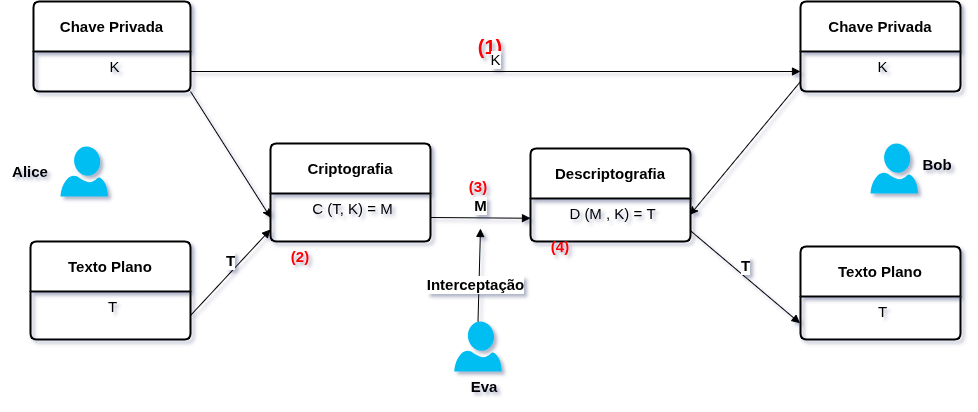
\includegraphics[scale=0.45]{algoritmo_simetrico.png}
	\caption{Funcionamento do algoritmo de criptografia simétrico}
	\label{fig:algoritmo_simetrico}
\end{figure}

A principal vantagem dos algoritmos de criptografia simétrica é sua eficiência e velocidade, especialmente em comparação com os algoritmos de criptografia assimétrica. No entanto, um dos desafios mais significativos é a distribuição segura da chave secreta. Se Eva conseguir interceptar ou descobrir a chave secreta, toda a comunicação entre Alice e Bob será comprometida.\\

Pelo motivo descrito acima, é essencial que Alice e Bob utilizem métodos seguros para compartilhar a chave secreta e garantam que ela permaneça protegida contra acessos não autorizados.

\subsection{A evolução: Key-Encryption-Key}

O conceito de Key-Encryption-Key, ou Chave de Criptografia de Chaves, é uma tecnologia utilizada para proteger outras chaves criptográficas, como por exemplo, o uso da KEK para proteger as Chaves de Criptografia de Dados(DEK). Ao usar uma KEK para resguardar as DEKs, adiciona-se uma camada extra de segurança ao sistema, melhorando significativamente sua proteção como um todo.\\

A Figura \ref{fig:kek} ilustra o funcionamento e da utilização do conceito KEK.

\begin{figure}[H]
	\centering
	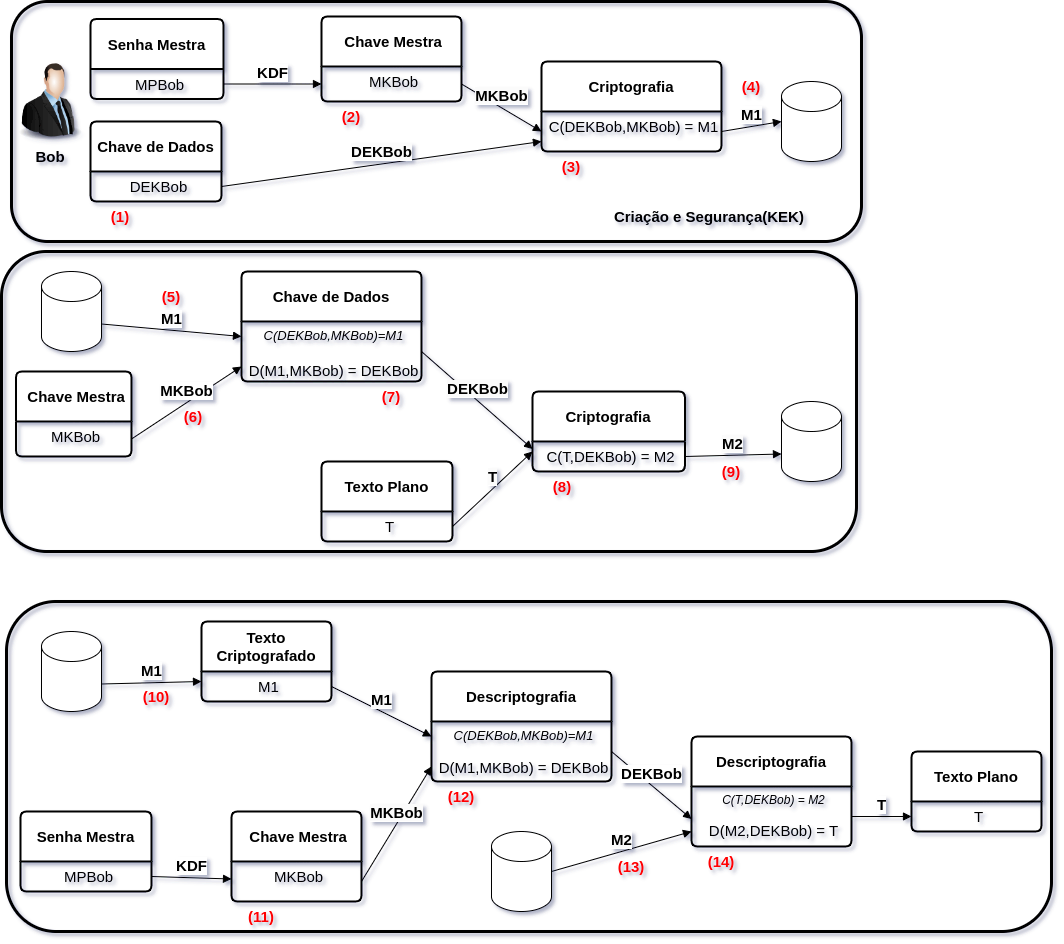
\includegraphics[scale=0.45]{kek.png}
	\caption{Funcionamento do conceito Key-Encryption-Key}
	\label{fig:kek}
\end{figure}

O Key-Encryption-Key é um componente essencial em arquiteturas de segurança que exigem a proteção de múltiplas chaves criptográficas \textbf{DEK}. Seu uso permite a proteção eficiente das DEKs, garantindo a segurança dos dados criptografados e simplificando a gestão das chaves. Implementar KEKs corretamente é necessário para manter a integridade e a confidencialidade dos dados em qualquer sistema seguro.\\

\pagebreak

% Página
\section{Segura Cofre: Aplicando Key-Encryption-Key na Prática}

\subsection{Arquitetura da Solução}

\subsection{Arquitetura da Solução}

\pagebreak

% Página
\section{Implementação e Melhores Práticas}


%Copyright
\vspace*{\fill}
\begin{flushright}
	\underline{\textit{Copyright}}\\
	All rights reserved to MT4 Tecnologia LTDA.\bigskip

	\underline{\textit{Propósito deste documento}}\\
	Segura Cofre e Key-Encryption-Key\bigskip
	
	\underline{\textit{MT4 Tecnologia Ltda.}}\\
	Rua Joaquim Antunes, 767 – Pinheiros – São Paulo\\
	Phone: +55 11 3065-7070\\
	\url{www.mt4.com.br}\\
	\href{mailto:support@segura.security}{support@segura.security}\\
\end{flushright}

\end{document}